\documentclass[10pt]{book}
\usepackage[utf8]{inputenc}
\usepackage[T2A]{fontenc}
\usepackage[russian]{babel}
\usepackage{amsmath,amssymb}
\usepackage{jeolm}
\usepackage{jeolm-tourn-limited}
\usepackage{parskip}
\usepackage{graphicx}
\usepackage{multicol}
\pagestyle{empty}

\usepackage{hyperref}
\hypersetup{
    colorlinks,
    citecolor=black,
    filecolor=black,
    linkcolor=black,
    urlcolor=black
}
% \usepackage[a5paper,margin=2em]{geometry}

% \usepackage{pgfpages}
\usepackage{epigraph}
%\pgfpagesuselayout{2 on 1}[a4paper,landscape]

%\def\jeolmleague{7 класс}

\makeatletter

\newcommand{\l@abcd}[2]{\hbox to\textwidth{#1 \dotfill\textbf{ #2}}}

\begin{document}

\begin{center}
	\Huge{\bf 32-я Летняя Многопредметная Школа}\\
	\Large{\bf 7 класс}\\ \vspace{.3cm}
	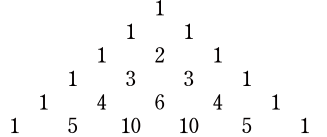
\includegraphics[width=\textwidth]{pasc}
	\begin{multicols}{2}
		Будимир Баев \\
		Владимир Брагин \\
		Надежда Власова \\
		Александр Смирнов \\
	\end{multicols}
\end{center}

\newpage

\begin{center}
На краю \\
Пучины дикой~--- зыбки, а быть может~--- \\
Могилы Мирозданья, где огня\\
И воздуха, материков, морей\\
В помине даже нет, но все они\\
В правеществе зачаточно кишат,\\
Смесившись и воюя меж собой,\\
Пока Творец Всевластный не велит\\
Им новые миры образовать;\\
У этой бездны осторожный Враг,\\
С порога Ада созерцая даль,\\
Обмысливал свой предстоящий путь...
\end{center}

\tableofcontents\newpage

\renewcommand{\@oddhead}{\vbox{\hbox to \textwidth{{\raisebox{1.8mm}{\strut{\small\bfseries Кировская ЛМШ 2016, 7 класс}}\hfil\raisebox{1.8mm}{\strut\bfseries\thepage}}}\hrule}}
\renewcommand{\@evenhead}{\vbox{\hbox to \textwidth{{\raisebox{1.8mm}{\strut\bfseries\thepage}\hfil\raisebox{1.8mm}{\strut{\small\bfseries Кировская ЛМШ 2016, 7 класс}}}}\hrule}}


\addcontentsline{toc}{abcd}{\bf Делимость. 4 июля}
\begin{center}
\textbf{\Large Делимость}\\
%\textit{Профи}\\
\textit{04.07.16}
\end{center}

\epigraph{\it Как зарплату делить будем? Поровну, по-честному, по-братски или по справедливости?}{@shhdup}

\begin{problems}
\item Пусть $a$~--- чётное число, не кратное $4$. Докажите, что разность $a^2 - 4$ делится на $32$.
\item Известно, что $5x+8y-1$ делится на $13$.\\ \textbf{a)} Докажите, что $5x+60y-1$ делится на $13$.\\ \textbf{b)} Найдите остаток от деления $18x-31y$ на $13$. \\ \textbf{c)} Найдите остаток от деления $x-y$ на $13$.
\item Вася написал на доске два числа, перемножил их и получил четырёхзначное число. После этого он заменил буквы на числа, причём разным числам соответствуют разные буквы. В итоге получилось $AB \cdot CD = EEFF$. Докажите, что Вася ошибся.
\item На очень большой и длинной доске записано число $11^{2016}$. Потом вместо этого числа записали сумму его цифр. Затем снова вместо полученного числа записали сумму его цифр. Этот процесс продолжается до тех пор, пока не останется однозначное число. Найдите это число. 
\item На доске записаны два числа: единица и двойка. Каждую минуту Маша умножает два самых больших числа, написанных на доске, прибавляет к ним $1$ и записывает полученное число на доску. Докажите, что Маша никогда не запишет число, делящееся на $4$.
\item Пусть $k>2$~--- нечётное натуральное число. Докажите, что для любого натурального $n$ число $1^{k^n}+2^{k^n}+...+(k-1)^{k^n}$ делится на $k$.
\item Может ли $5^n-1$ делиться на $4^n-1$ при натуральном $n$? 
\item В ряд записана последовательность чисел $a_n$, причём оказалось, что для любого числа, начиная с третьего, справедлива формула $a_n=a_{n-2}+2a_{n-1}$. Оказалось, что первые два члена~--- простые числа. Какое максимальное количество подряд идущих простых чисел может еще встретиться после них?
%\item Можно ли числа $1, 2, 3, . . . , 20$ так расставить в вершинах и серединах ребер куба так, чтобы каждое число, стоящее в середине ребра, равнялось полусумме чисел на концах этого ребра? (не совсем делимость, халява)
% \item Назовем число $n$ \textit{удобным}, если $n^2+1$ делится на $1000001$. Докажите, что среди чисел $1, 2, ..., 1000000$ четное число удобных.
% \item Назовем число совершенно простым, если оно простое и если при любой перестановке его цифр снова получается простое число. Докажите, что в записи абсолютно простого числа не может содержаться более трех различных цифр.
% \item Из трех различных цифр составили шесть различных двузначных чисел (каждая цифра входит в запись по одному разу). Докажите, что если сложить какие-то три из этих чисел и вычесть сумму трех оставшихся, то полученный ответ будет делиться на $18$. 

\end{problems}

\resetproblem
\vspace{1cm}
\newpage
\addcontentsline{toc}{abcd}{\bf Вступительная олимпиада. 4 июля}
\begin{center}
\textbf{\Large Вступительная олимпиада}\\
%\textit{Профи}\\
\textit{04.07.16}
\end{center}


\begin{problems}

\item На острове Мадагаскар есть Холм и Озеро. Глория идет от Холма к Озеру, а навстречу ей от Озера бежит Алекс. Известно, что Глория проходит этот путь за 5 часов, а Алекс всего за час. Через 50 минут после встречи Глории и Алекса Марти также прошел от Озера к Холму, причем это расстояние Марти проходил 1 час 40 минут. Через сколько минут после встречи с Глорией Марти дойдет до Холма, если Глория и Алекс начали движение одновременно? Ответ обоснуйте.

%\item Вася и Петя получили от своих родителей по 100 рублей и решили покататься по городу. Вася катался на маршрутках за 17 и за 10 рублей, а Петя~--- на автобусах за 12 рублей. К вечеру оказалось, что они поездили одинаковое количество раз и потратили одинаковое количество денег. Сколько у них осталось?

%\item На главной диагонали шашечной доски $10\times 10$ стоит 10 шашек (все в разных клетках). За один ход разрешается взять любую пару шашек и передвинуть каждую из них на одну клетку вниз. Можно ли за несколько ходов поставить все шашки на нижнюю горизонталь?

%\item На столе в виде треугольника выложены 28 монет одинакового размера (рис.). Известно, что суммарная масса любой тройки монет, которые попарно касаются друг друга, равна 10  г. Найдите суммарную массу всех 18  монет на границе треугольника.
%\begin{figure}[h!]
%\center{\includegraphics[scale=0.5]{coins.png}}
%\end{figure}\\

\item Натуральные числа от 1 до 20 расставили по кругу в некотором порядке, а затем покрасили в красный цвет те из них, которые являются делителями своего правого соседа. Какое наибольшее количество красных чисел могло получиться?

\item В выпуклом пятиугольнике $ABCDE$ углы $ABC$ и $CDE$ равны, $AB=ED$, $BC=CD$. Докажите, что отрезки $AD$ и $BE$ равны.

\item Пусть $d_1, d_2 , d_3$ и $d_4$~--- наименьшие различные делители натурального числа $n$. Оказалось, что $d_1^2+d_2^2+d_3^2+d_4^2=n$. Чему могло быть равно $n$ (укажите все варианты)?

\item Если в детектор фальшивых монет опустить 5 монет весом $a, b, c, d, e$ граммов, где $a<b<c<d<e$, то он сбросит монеты весом $b$ и $c$ граммов в правую чашу, а остальные в левую. Есть 50 монет попарно различных по весу, они пронумерованы и легко различаются по внешнему виду. Как при помощи детектора определить самую легкую монету?

\item На острове рыцарей (которые говорят только правду) и лжецов (которые всегда
лгут) состоялся шахматный фестиваль. 64 любителя шахмат встали по
одному на клетки большой шахматной доски. После этого каждый сказал:
``{\it Среди людей, стоящих со мной на одной горизонтали, больше лжецов, чем
среди людей, стоящих со мной на одной вертикали}''. Докажите, что
количество рыцарей делится на~8.

\end{problems}

\resetproblem
\vspace{1cm}
\newpage
\addcontentsline{toc}{abcd}{\bf Геометрические неравенства. 5 июля}
\begin{center}
\Large
\textbf{Геометрические неравенства. 05 июля.}
\end{center}  
\large
\begin{enumerate}

\item (тестовая, на знание двух теорем) На стороне $AB$ четырёхугольника $ABCD$ отмечена точка $E$ такая, что $\angle DEA+\angle DBA = 180^{\circ}$. Докажите, что $BC+DE>CD$.

$\textit{Теоретические}$

\item В треугольнике напротив наибольшей стороны угол равен $60^{\circ}$. Чему равны два других угла?

\item На плоскости отмечены точки $A_{1}, A_{2},..., A_{n}$, где $n\geq 3$. Докажите, что $A_{1}A_{2}+A_{2}A_{3}+...+A_{n-1}A_{n}\geq A_{1}A_{n}$. Когда достигается равенство?

\item Отрезки $AC$ и $BD$ пересекаются. Докажите, что $AB+CD<AC+BD$.

\item а) Точки $M$ и $N$ расположены по одну сторону от прямой $\ell$. Постройте на прямой $\ell$ такую точку $K$, чтобы сумма $MK+NK$ была наименьшей. \\
б) Точки $M$ и $N$ расположены по разные стороны от пары параллельных прямых. Постройте на прямых точки $A$ и $B$, так чтобы отрезок $AB$ был перпендикулярен прямым, а сумма отрезков $MA$, $AB$ и $BK$ была наименьшей.\\
в) Точка $M$ лежит внутри острого угла. Постройте на сторонах этого угла точки $A$ и $B$, для которых периметр треугольника $AMB$ был бы наименьшим.

\item а) В треугольнике $ABC$ отмечена точка $T$. Докажите, что $AT+CT<AB+CB$.\\
б) Внутри треугольника $ABC$ расположен треугольник $A_{1}B_{1}C_{1}$. Докажите, что его периметр меньше периметра треугольника $ABC$.\\
в) Внутри выпуклого многоугольника $A_{1}A_{2}...A_{n}$ расположен выпуклый многоугольник $B_{1}B_{2}...B_{m}$. Докажите, что периметр внутреннего многоугольника меньше периметра наружного.

\item В треугольнике $ABC$ отмечена произвольная точка $T$. Докажите, что $AT+BT+CT$ больше полупериметра и меньше периметра треугольника $ABC$. 

$\textit{Более сложные геометрические неравенства}$

\item На стороне $AB$ треугольника $ABC$ отмечена такая точка $D$, что
$AB = CD$. Докажите, что $BC > AD$.

\item Пусть $a, b, c$ — длины сторон треугольника, $m_{a},m_{b},m_{c}$ --- длины опущенных на эти стороны медиан и $p=\frac{a+b+c}{2}$
--- полупериметр данного треугольника. Докажите, что $m_{a}+m_{b}+m_{c}>p$.

\item На основании $AC$ равнобедренного треугольника $ABC$ отметили точку $D$, а на продолжении стороны $AC$ за точку $C$ -- точку $E$ таким образом, что $AD=CE$. Докажите, что $BD+BE>BA+BC$.

\item Отрезки $AA_{1}$ и $BB_{1}$ — биссектрисы треугольника $ABC$. Докажите, что a) $AB_{1} < AB$; б) $A_{1}B_{1} < AB$. 

\item В треугольнике $ABC$ провели биссектрису $CK$, а в треугольнике $CKB$ провели биссектрису $KL$. Прямые $KL$ и $AC$ пересеклись в точке $M$. Известно, что $\angle CAB > \angle BCA$. Докажите, что $AK+KC>AM$.

\end{enumerate}
\resetproblem
\vspace{1cm}
\newpage

\end{document}